%%%%%%%%%%%%%%%%%%%%%%%%%%%%%%%%%%%%%%%%%%%%%%%%%%%%%%%%%%%%%%%
%
% Welcome to writeLaTeX --- just edit your LaTeX on the left,
% and we'll compile it for you on the right. If you give
% someone the link to this page, they can edit at the same
% time. See the help menu above for more info. Enjoy!
%
%%%%%%%%%%%%%%%%%%%%%%%%%%%%%%%%%%%%%%%%%%%%%%%%%%%%%%%%%%%%%%%

% --------------------------------------------------------------
% This is all preamble stuff that you don't have to worry about.
% Head down to where it says "Start here"
% --------------------------------------------------------------
 
\documentclass[12pt]{article}
 
\usepackage[margin=1in]{geometry}
\usepackage{amsmath,amsthm,amssymb}

\usepackage{listings}
\usepackage{xcolor}

\usepackage{tikz}
\usetikzlibrary{shapes,positioning}

\tikzset{ell/.style={circle,draw,minimum height=0.5cm,minimum width=0.5cm,inner sep=0.2cm}}

%New colors defined below
\definecolor{codegreen}{rgb}{0,0.6,0}
\definecolor{codegray}{rgb}{0.5,0.5,0.5}
\definecolor{codepurple}{rgb}{0.58,0,0.82}
\definecolor{backcolour}{rgb}{0.95,0.95,0.92}

%Code listing style named "mystyle"
\lstdefinestyle{mystyle}{
  backgroundcolor=\color{backcolour}, commentstyle=\color{codegreen},
  keywordstyle=\color{magenta},
  numberstyle=\tiny\color{codegray},
  stringstyle=\color{codepurple},
  basicstyle=\ttfamily\footnotesize,
  breakatwhitespace=false,         
  breaklines=true,                 
  captionpos=b,                    
  keepspaces=true,                 
  numbers=left,                    
  numbersep=5pt,                  
  showspaces=false,                
  showstringspaces=false,
  showtabs=false,                  
  tabsize=2
}

%"mystyle" code listing set
\lstset{style=mystyle}

 
\newcommand{\N}{\mathbb{N}}
\newcommand{\Z}{\mathbb{Z}}
 
\newenvironment{theorem}[2][Theorem]{\begin{trivlist}
\item[\hskip \labelsep {\bfseries #1}\hskip \labelsep {\bfseries #2.}]}{\end{trivlist}}
\newenvironment{lemma}[2][Lemma]{\begin{trivlist}
\item[\hskip \labelsep {\bfseries #1}\hskip \labelsep {\bfseries #2.}]}{\end{trivlist}}
\newenvironment{exercise}[2][Exercise]{\begin{trivlist}
\item[\hskip \labelsep {\bfseries #1}\hskip \labelsep {\bfseries #2.}]}{\end{trivlist}}
\newenvironment{problem}[2][Problem]{\begin{trivlist}
\item[\hskip \labelsep {\bfseries #1}\hskip \labelsep {\bfseries #2.}]}{\end{trivlist}}
\newenvironment{question}[2][Question]{\begin{trivlist}
\item[\hskip \labelsep {\bfseries #1}\hskip \labelsep {\bfseries #2.}]}{\end{trivlist}}
\newenvironment{corollary}[2][Corollary]{\begin{trivlist}
\item[\hskip \labelsep {\bfseries #1}\hskip \labelsep {\bfseries #2.}]}{\end{trivlist}}

\newenvironment{solution}{\begin{proof}[Solution]}{\end{proof}}
 
\begin{document}
 
% --------------------------------------------------------------
%                         Start here
% --------------------------------------------------------------
 
\title{Homework 1}%replace X with the appropriate number
\author{Mengxiang Jiang\\ %replace with your name
CSEN 5336 Analysis of Algorithms} %if necessary, replace with your course title
 
\maketitle
 
\begin{problem}{1} %You can use theorem, exercise, problem, or question here.  Modify x.yz to be whatever number you are proving
    Illustrate the operation of RADIX-SORT on the following list of English words: COW, DOG, TOW,
    RUG, ROW, HUG, MOB, FOX, TAB, BAR, CAR, FUR\\\\
    Assuming standard lexicographic (alphabetic) ordering for the sort.\\
    Iterations:\\
    1:MO\underline{B}, TA\underline{B}, DO\underline{G}, HU\underline{G}, BA\underline{R}, CA\underline{R}, FU\underline{R}, CO\underline{W}, TO\underline{W}, RO\underline{W}, FO\underline{X}\\\\
    2:T\underline{A}B, B\underline{A}R, C\underline{A}R, M\underline{O}B, D\underline{O}G, C\underline{O}W, T\underline{O}W, R\underline{O}W, F\underline{O}X, H\underline{U}G, F\underline{U}R\\\\
    3:\underline{B}AR, \underline{C}AR, \underline{C}OW, \underline{D}OG, \underline{F}OX, \underline{F}UR, \underline{H}UG, \underline{M}OB, \underline{R}OW, \underline{T}AB, \underline{T}OW
\end{problem}

\begin{problem}{2} %You can use theorem, exercise, problem, or question here.  Modify x.yz to be whatever number you are proving
    Use the procedure MAX-HEAPIFY in a bottom-up manner to convert the array
    A = $<1, 4, 3, 5, 8, 9, 0, 7, 2, 6>$ to build a max heap    
    
    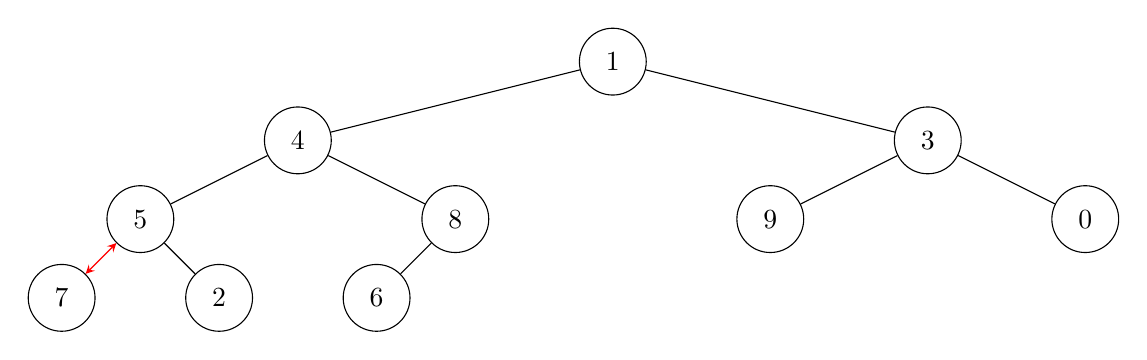
\begin{tikzpicture}[>=stealth]
        \node[ell] (a)at (8,3) {1};
        \node[ell] (b)at (4,2) {4};
        \node[ell] (c)at (12,2) {3};
        \node[ell] (d)at (2,1) {5};
        \node[ell] (e)at (6,1) {8};
        \node[ell] (f)at (10,1) {9};
        \node[ell] (g)at (14,1) {0};
        \node[ell] (h)at (1,0) {7};
        \node[ell] (i)at (3,0) {2};
        \node[ell] (j)at (5,0) {6};

        \draw [] (a) to []node[]{} (b);
        \draw [] (a) to []node[]{} (c);
        \draw [] (b) to []node[]{} (d);
        \draw [] (b) to []node[]{} (e);
        \draw [] (c) to []node[]{} (f);
        \draw [] (c) to []node[]{} (g);
        \draw [red,<->] (d) to []node[]{} (h);
        \draw [] (d) to []node[]{} (i);
        \draw [] (e) to []node[]{} (j);
    \end{tikzpicture}

    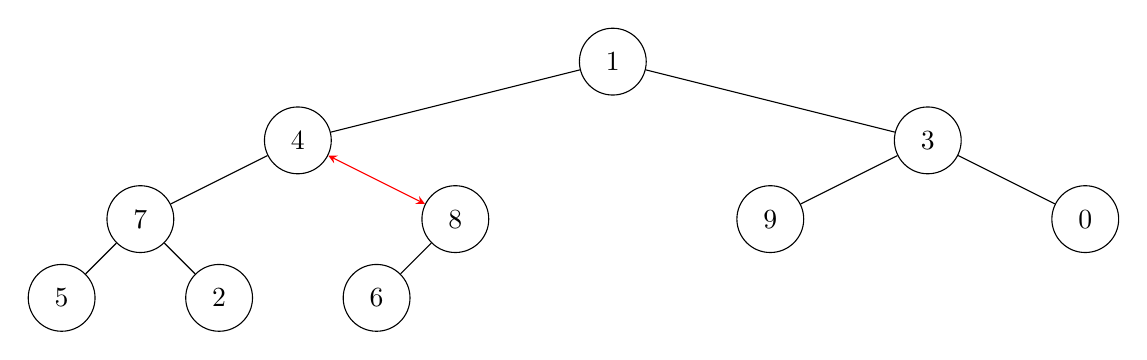
\begin{tikzpicture}[>=stealth]
        \node[ell] (a)at (8,3) {1};
        \node[ell] (b)at (4,2) {4};
        \node[ell] (c)at (12,2) {3};
        \node[ell] (d)at (2,1) {7};
        \node[ell] (e)at (6,1) {8};
        \node[ell] (f)at (10,1) {9};
        \node[ell] (g)at (14,1) {0};
        \node[ell] (h)at (1,0) {5};
        \node[ell] (i)at (3,0) {2};
        \node[ell] (j)at (5,0) {6};

        \draw [] (a) to []node[]{} (b);
        \draw [] (a) to []node[]{} (c);
        \draw [] (b) to []node[]{} (d);
        \draw [red,<->] (b) to []node[]{} (e);
        \draw [] (c) to []node[]{} (f);
        \draw [] (c) to []node[]{} (g);
        \draw [] (d) to []node[]{} (h);
        \draw [] (d) to []node[]{} (i);
        \draw [] (e) to []node[]{} (j);
    \end{tikzpicture}

    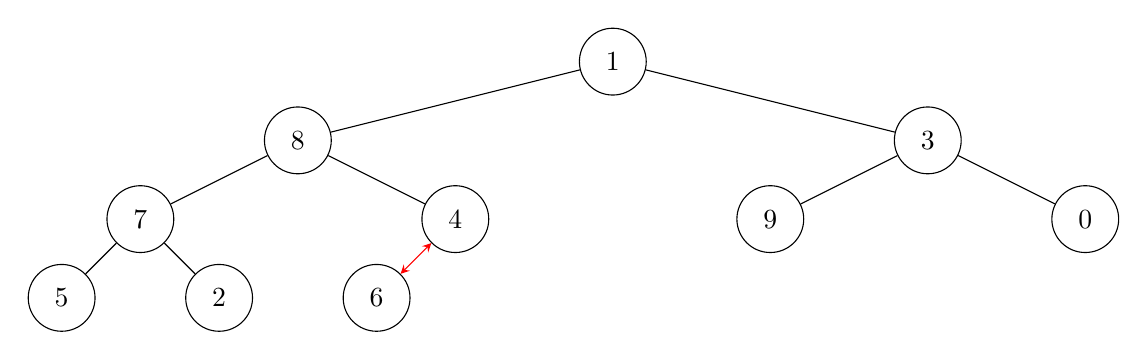
\begin{tikzpicture}[>=stealth]
        \node[ell] (a)at (8,3) {1};
        \node[ell] (b)at (4,2) {8};
        \node[ell] (c)at (12,2) {3};
        \node[ell] (d)at (2,1) {7};
        \node[ell] (e)at (6,1) {4};
        \node[ell] (f)at (10,1) {9};
        \node[ell] (g)at (14,1) {0};
        \node[ell] (h)at (1,0) {5};
        \node[ell] (i)at (3,0) {2};
        \node[ell] (j)at (5,0) {6};

        \draw [] (a) to []node[]{} (b);
        \draw [] (a) to []node[]{} (c);
        \draw [] (b) to []node[]{} (d);
        \draw [] (b) to []node[]{} (e);
        \draw [] (c) to []node[]{} (f);
        \draw [] (c) to []node[]{} (g);
        \draw [] (d) to []node[]{} (h);
        \draw [] (d) to []node[]{} (i);
        \draw [red,<->] (e) to []node[]{} (j);
    \end{tikzpicture}

    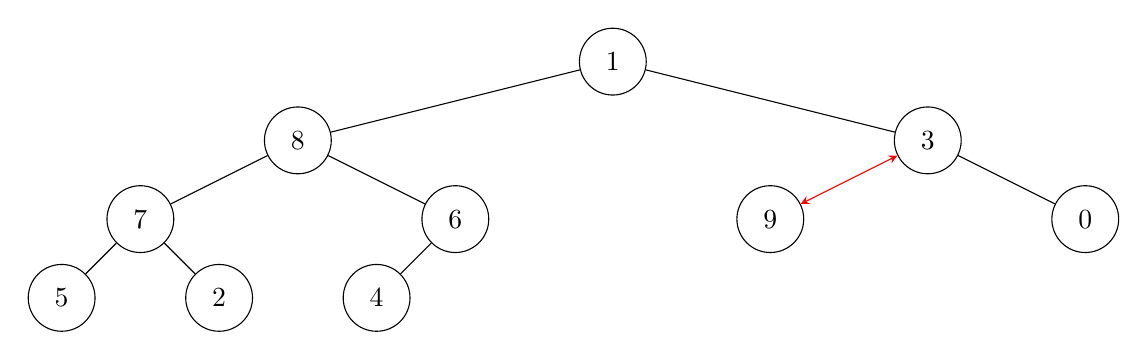
\begin{tikzpicture}[>=stealth]
        \node[ell] (a)at (8,3) {1};
        \node[ell] (b)at (4,2) {8};
        \node[ell] (c)at (12,2) {3};
        \node[ell] (d)at (2,1) {7};
        \node[ell] (e)at (6,1) {6};
        \node[ell] (f)at (10,1) {9};
        \node[ell] (g)at (14,1) {0};
        \node[ell] (h)at (1,0) {5};
        \node[ell] (i)at (3,0) {2};
        \node[ell] (j)at (5,0) {4};

        \draw [] (a) to []node[]{} (b);
        \draw [] (a) to []node[]{} (c);
        \draw [] (b) to []node[]{} (d);
        \draw [] (b) to []node[]{} (e);
        \draw [red,<->] (c) to []node[]{} (f);
        \draw [] (c) to []node[]{} (g);
        \draw [] (d) to []node[]{} (h);
        \draw [] (d) to []node[]{} (i);
        \draw [] (e) to []node[]{} (j);
    \end{tikzpicture}

    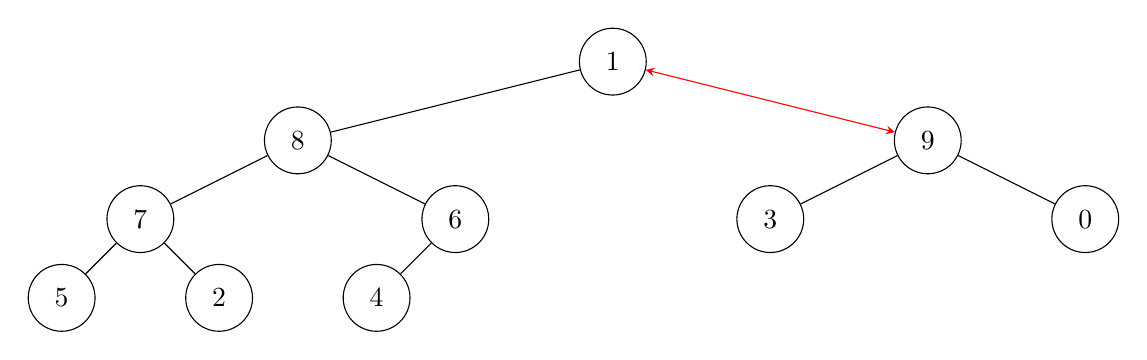
\begin{tikzpicture}[>=stealth]
        \node[ell] (a)at (8,3) {1};
        \node[ell] (b)at (4,2) {8};
        \node[ell] (c)at (12,2) {9};
        \node[ell] (d)at (2,1) {7};
        \node[ell] (e)at (6,1) {6};
        \node[ell] (f)at (10,1) {3};
        \node[ell] (g)at (14,1) {0};
        \node[ell] (h)at (1,0) {5};
        \node[ell] (i)at (3,0) {2};
        \node[ell] (j)at (5,0) {4};

        \draw [] (a) to []node[]{} (b);
        \draw [red,<->] (a) to []node[]{} (c);
        \draw [] (b) to []node[]{} (d);
        \draw [] (b) to []node[]{} (e);
        \draw [] (c) to []node[]{} (f);
        \draw [] (c) to []node[]{} (g);
        \draw [] (d) to []node[]{} (h);
        \draw [] (d) to []node[]{} (i);
        \draw [] (e) to []node[]{} (j);
    \end{tikzpicture}

    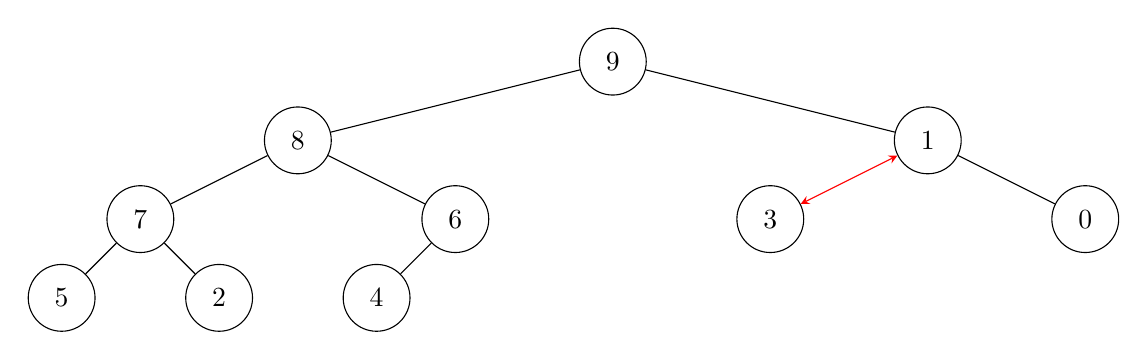
\begin{tikzpicture}[>=stealth]
        \node[ell] (a)at (8,3) {9};
        \node[ell] (b)at (4,2) {8};
        \node[ell] (c)at (12,2) {1};
        \node[ell] (d)at (2,1) {7};
        \node[ell] (e)at (6,1) {6};
        \node[ell] (f)at (10,1) {3};
        \node[ell] (g)at (14,1) {0};
        \node[ell] (h)at (1,0) {5};
        \node[ell] (i)at (3,0) {2};
        \node[ell] (j)at (5,0) {4};

        \draw [] (a) to []node[]{} (b);
        \draw [] (a) to []node[]{} (c);
        \draw [] (b) to []node[]{} (d);
        \draw [] (b) to []node[]{} (e);
        \draw [red,<->] (c) to []node[]{} (f);
        \draw [] (c) to []node[]{} (g);
        \draw [] (d) to []node[]{} (h);
        \draw [] (d) to []node[]{} (i);
        \draw [] (e) to []node[]{} (j);
    \end{tikzpicture}

    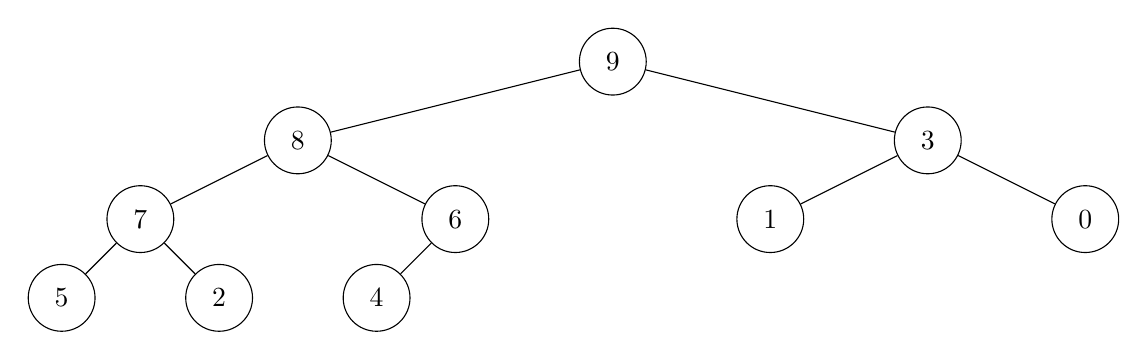
\begin{tikzpicture}[>=stealth]
        \node[ell] (a)at (8,3) {9};
        \node[ell] (b)at (4,2) {8};
        \node[ell] (c)at (12,2) {3};
        \node[ell] (d)at (2,1) {7};
        \node[ell] (e)at (6,1) {6};
        \node[ell] (f)at (10,1) {1};
        \node[ell] (g)at (14,1) {0};
        \node[ell] (h)at (1,0) {5};
        \node[ell] (i)at (3,0) {2};
        \node[ell] (j)at (5,0) {4};

        \draw [] (a) to []node[]{} (b);
        \draw [] (a) to []node[]{} (c);
        \draw [] (b) to []node[]{} (d);
        \draw [] (b) to []node[]{} (e);
        \draw [] (c) to []node[]{} (f);
        \draw [] (c) to []node[]{} (g);
        \draw [] (d) to []node[]{} (h);
        \draw [] (d) to []node[]{} (i);
        \draw [] (e) to []node[]{} (j);
    \end{tikzpicture}

    Resulting array is $<9,8,3,7,6,1,0,5,2,4>$.

\end{problem}
\pagebreak
\begin{problem}{3}
Insert the following set of keys {1, 4, 3, 5, 8, 9, 0, 7, 2, 6} in an empty binary search tree in the
order they are listed.\\\\
After adding 1\\
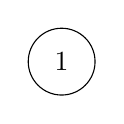
\begin{tikzpicture}[>=stealth]
    \node[ell] (a)at (8,3) {1};
\end{tikzpicture}
\\\\After adding 4\\\\
\begin{tikzpicture}[>=stealth]
    \node[ell] (a)at (8,3) {1};
    \node[ell] (b)at (12,2) {4};

    \draw [] (a) to []node[]{} (b);
\end{tikzpicture}
\\\\After adding 3\\\\
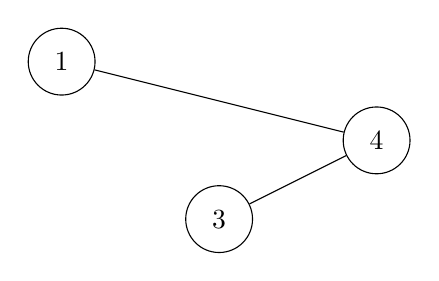
\begin{tikzpicture}[>=stealth]
    \node[ell] (a)at (8,3) {1};
    \node[ell] (b)at (12,2) {4};
    \node[ell] (c)at (10,1) {3};

    \draw [] (a) to []node[]{} (b);
    \draw [] (b) to []node[]{} (c);
\end{tikzpicture}
\\\\After adding 5\\\\
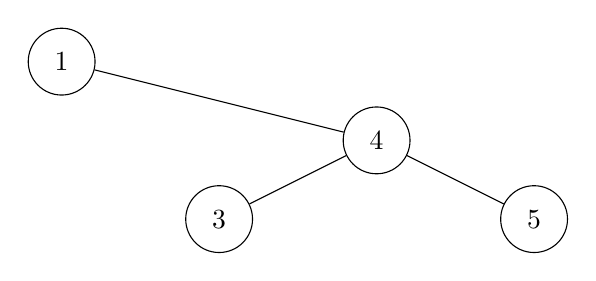
\begin{tikzpicture}[>=stealth]
    \node[ell] (a)at (8,3) {1};
    \node[ell] (b)at (12,2) {4};
    \node[ell] (c)at (10,1) {3};
    \node[ell] (d)at (14,1) {5};

    \draw [] (a) to []node[]{} (b);
    \draw [] (b) to []node[]{} (c);
    \draw [] (b) to []node[]{} (d);
\end{tikzpicture}
\\\\After adding 8\\\\
\begin{tikzpicture}[>=stealth]
    \node[ell] (a)at (8,3) {1};
    \node[ell] (b)at (12,2) {4};
    \node[ell] (c)at (10,1) {3};
    \node[ell] (d)at (14,1) {5};
    \node[ell] (e)at (15,0) {8};

    \draw [] (a) to []node[]{} (b);
    \draw [] (b) to []node[]{} (c);
    \draw [] (b) to []node[]{} (d);
    \draw [] (d) to []node[]{} (e);
\end{tikzpicture}
\pagebreak
\\\\After adding 9\\\\
\begin{tikzpicture}[>=stealth]
    \node[ell] (a)at (8,3) {1};
    \node[ell] (b)at (12,2) {4};
    \node[ell] (c)at (10,1) {3};
    \node[ell] (d)at (14,1) {5};
    \node[ell] (e)at (15,0) {8};
    \node[ell] (f)at (15.5,-1) {9};

    \draw [] (a) to []node[]{} (b);
    \draw [] (b) to []node[]{} (c);
    \draw [] (b) to []node[]{} (d);
    \draw [] (d) to []node[]{} (e);
    \draw [] (e) to []node[]{} (f);
\end{tikzpicture}
\\\\After adding 0\\\\
\begin{tikzpicture}[>=stealth]
    \node[ell] (a)at (8,3) {1};
    \node[ell] (b)at (12,2) {4};
    \node[ell] (c)at (10,1) {3};
    \node[ell] (d)at (14,1) {5};
    \node[ell] (e)at (15,0) {8};
    \node[ell] (f)at (15.5,-1) {9};
    \node[ell] (g)at (4,2) {0};

    \draw [] (a) to []node[]{} (b);
    \draw [] (b) to []node[]{} (c);
    \draw [] (b) to []node[]{} (d);
    \draw [] (d) to []node[]{} (e);
    \draw [] (e) to []node[]{} (f);
    \draw [] (a) to []node[]{} (g);
\end{tikzpicture}
\\\\After adding 7\\\\
\begin{tikzpicture}[>=stealth]
    \node[ell] (a)at (8,3) {1};
    \node[ell] (b)at (12,2) {4};
    \node[ell] (c)at (10,1) {3};
    \node[ell] (d)at (14,1) {5};
    \node[ell] (e)at (15,0) {8};
    \node[ell] (f)at (15.5,-1) {9};
    \node[ell] (g)at (4,2) {0};
    \node[ell] (h)at (14.5,-1) {7};

    \draw [] (a) to []node[]{} (b);
    \draw [] (b) to []node[]{} (c);
    \draw [] (b) to []node[]{} (d);
    \draw [] (d) to []node[]{} (e);
    \draw [] (e) to []node[]{} (f);
    \draw [] (a) to []node[]{} (g);
    \draw [] (e) to []node[]{} (h);
\end{tikzpicture}
\pagebreak
\\\\After adding 2\\\\
\begin{tikzpicture}[>=stealth]
    \node[ell] (a)at (8,3) {1};
    \node[ell] (b)at (12,2) {4};
    \node[ell] (c)at (10,1) {3};
    \node[ell] (d)at (14,1) {5};
    \node[ell] (e)at (15,0) {8};
    \node[ell] (f)at (15.5,-1) {9};
    \node[ell] (g)at (4,2) {0};
    \node[ell] (h)at (14.5,-1) {7};
    \node[ell] (i)at (9,0) {2};

    \draw [] (a) to []node[]{} (b);
    \draw [] (b) to []node[]{} (c);
    \draw [] (b) to []node[]{} (d);
    \draw [] (d) to []node[]{} (e);
    \draw [] (e) to []node[]{} (f);
    \draw [] (a) to []node[]{} (g);
    \draw [] (e) to []node[]{} (h);
    \draw [] (c) to []node[]{} (i);
\end{tikzpicture}
\\\\After adding 6\\\\
\begin{tikzpicture}[>=stealth]
    \node[ell] (a)at (8,3) {1};
    \node[ell] (b)at (12,2) {4};
    \node[ell] (c)at (10,1) {3};
    \node[ell] (d)at (14,1) {5};
    \node[ell] (e)at (15,0) {8};
    \node[ell] (f)at (15.5,-1) {9};
    \node[ell] (g)at (4,2) {0};
    \node[ell] (h)at (14.5,-1) {7};
    \node[ell] (i)at (9,0) {2};
    \node[ell] (j)at (14.25,-2) {6};

    \draw [] (a) to []node[]{} (b);
    \draw [] (b) to []node[]{} (c);
    \draw [] (b) to []node[]{} (d);
    \draw [] (d) to []node[]{} (e);
    \draw [] (e) to []node[]{} (f);
    \draw [] (a) to []node[]{} (g);
    \draw [] (e) to []node[]{} (h);
    \draw [] (c) to []node[]{} (i);
    \draw [] (h) to []node[]{} (j);
\end{tikzpicture}
\end{problem}

\begin{problem}{4}
Insert the following set of keys {1, 4, 3, 5, 8, 9, 0, 7, 2, 6} in an empty red-black tree in the order
they are listed.\\\\
After adding 1\\
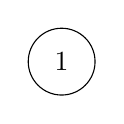
\begin{tikzpicture}[>=stealth]
    \node[ell] (a)at (8,3) {1};
\end{tikzpicture}
\\\\After adding 4\\\\
\begin{tikzpicture}[>=stealth]
    \node[ell] (a)at (8,3) {1};
    \node[red,ell] (b)at (12,2) {4};

    \draw [] (a) to []node[]{} (b);
\end{tikzpicture}
\pagebreak
\\\\After adding 3\\\\
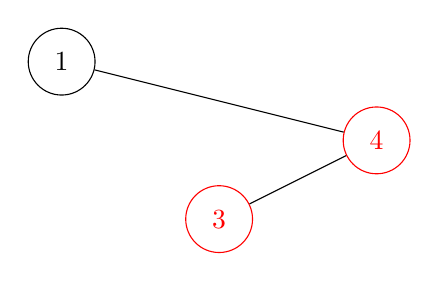
\begin{tikzpicture}[>=stealth]
    \node[ell] (a)at (8,3) {1};
    \node[red,ell] (b)at (12,2) {4};
    \node[red,ell] (c)at (10,1) {3};

    \draw [] (a) to []node[]{} (b);
    \draw [] (b) to []node[]{} (c);
\end{tikzpicture}
\\\\Case 5, right rotate on z.p\\\\
\begin{tikzpicture}[>=stealth]
    \node[ell] (a)at (8,3) {1};
    \node[red,ell] (b)at (12,2) {3};
    \node[red,ell] (c)at (14,1) {4};

    \draw [] (a) to []node[]{} (b);
    \draw [] (b) to []node[]{} (c);
\end{tikzpicture}
\\\\Case 4, change color of z.p and z.p.p and left rotate on z.p.p\\\\
\begin{tikzpicture}[>=stealth]
    \node[ell] (a)at (8,3) {3};
    \node[red,ell] (b)at (4,2) {1};
    \node[red,ell] (c)at (12,2) {4};

    \draw [] (a) to []node[]{} (b);
    \draw [] (a) to []node[]{} (c);
\end{tikzpicture}
\\\\After adding 5\\\\
\begin{tikzpicture}[>=stealth]
    \node[ell] (a)at (8,3) {3};
    \node[red,ell] (b)at (4,2) {1};
    \node[red,ell] (c)at (12,2) {4};
    \node[red,ell] (d)at (14,1) {5};

    \draw [] (a) to []node[]{} (b);
    \draw [] (a) to []node[]{} (c);
    \draw [] (c) to []node[]{} (d);
\end{tikzpicture}
\\\\Case 1, change color of z.p, y, z.p.p\\\\
\begin{tikzpicture}[>=stealth]
    \node[ell] (a)at (8,3) {3};
    \node[ell] (b)at (4,2) {1};
    \node[ell] (c)at (12,2) {4};
    \node[red,ell] (d)at (14,1) {5};

    \draw [] (a) to []node[]{} (b);
    \draw [] (a) to []node[]{} (c);
    \draw [] (c) to []node[]{} (d);
\end{tikzpicture}
\pagebreak
\\\\After adding 8\\\\
\begin{tikzpicture}[>=stealth]
    \node[ell] (a)at (8,3) {3};
    \node[ell] (b)at (4,2) {1};
    \node[ell] (c)at (12,2) {4};
    \node[red,ell] (d)at (14,1) {5};
    \node[red,ell] (e)at (15,0) {8};

    \draw [] (a) to []node[]{} (b);
    \draw [] (a) to []node[]{} (c);
    \draw [] (c) to []node[]{} (d);
    \draw [] (d) to []node[]{} (e);
\end{tikzpicture}
\\\\Case 4, change color of z.p and z.p.p and left rotate on z.p.p\\\\
\begin{tikzpicture}[>=stealth]
    \node[ell] (a)at (8,3) {3};
    \node[ell] (b)at (4,2) {1};
    \node[ell] (c)at (12,2) {5};
    \node[red,ell] (d)at (10,1) {4};
    \node[red,ell] (e)at (14,1) {8};

    \draw [] (a) to []node[]{} (b);
    \draw [] (a) to []node[]{} (c);
    \draw [] (c) to []node[]{} (d);
    \draw [] (c) to []node[]{} (e);
\end{tikzpicture}
\\\\After adding 9\\\\
\begin{tikzpicture}[>=stealth]
    \node[ell] (a)at (8,3) {3};
    \node[ell] (b)at (4,2) {1};
    \node[ell] (c)at (12,2) {5};
    \node[red,ell] (d)at (10,1) {4};
    \node[red,ell] (e)at (14,1) {8};
    \node[red,ell] (f)at (15,0) {9};

    \draw [] (a) to []node[]{} (b);
    \draw [] (a) to []node[]{} (c);
    \draw [] (c) to []node[]{} (d);
    \draw [] (c) to []node[]{} (e);
    \draw [] (e) to []node[]{} (f);
\end{tikzpicture}
\\\\Case 1, change color of z.p, y, z.p.p\\\\
\begin{tikzpicture}[>=stealth]
    \node[ell] (a)at (8,3) {3};
    \node[ell] (b)at (4,2) {1};
    \node[red,ell] (c)at (12,2) {5};
    \node[ell] (d)at (10,1) {4};
    \node[ell] (e)at (14,1) {8};
    \node[red,ell] (f)at (15,0) {9};

    \draw [] (a) to []node[]{} (b);
    \draw [] (a) to []node[]{} (c);
    \draw [] (c) to []node[]{} (d);
    \draw [] (c) to []node[]{} (e);
    \draw [] (e) to []node[]{} (f);
\end{tikzpicture}
\pagebreak
\\\\After adding 0\\\\
\begin{tikzpicture}[>=stealth]
    \node[ell] (a)at (8,3) {3};
    \node[ell] (b)at (4,2) {1};
    \node[red,ell] (c)at (12,2) {5};
    \node[ell] (d)at (10,1) {4};
    \node[ell] (e)at (14,1) {8};
    \node[red,ell] (f)at (15,0) {9};
    \node[red,ell] (g)at (2,1) {0};

    \draw [] (a) to []node[]{} (b);
    \draw [] (a) to []node[]{} (c);
    \draw [] (c) to []node[]{} (d);
    \draw [] (c) to []node[]{} (e);
    \draw [] (e) to []node[]{} (f);
    \draw [] (b) to []node[]{} (g);
\end{tikzpicture}
\\\\After adding 7\\\\
\begin{tikzpicture}[>=stealth]
    \node[ell] (a)at (8,3) {3};
    \node[ell] (b)at (4,2) {1};
    \node[red,ell] (c)at (12,2) {5};
    \node[ell] (d)at (10,1) {4};
    \node[ell] (e)at (14,1) {8};
    \node[red,ell] (f)at (15,0) {9};
    \node[red,ell] (g)at (2,1) {0};
    \node[red,ell] (h)at (13,0) {7};

    \draw [] (a) to []node[]{} (b);
    \draw [] (a) to []node[]{} (c);
    \draw [] (c) to []node[]{} (d);
    \draw [] (c) to []node[]{} (e);
    \draw [] (e) to []node[]{} (f);
    \draw [] (b) to []node[]{} (g);
    \draw [] (e) to []node[]{} (h);
\end{tikzpicture}
\\\\After adding 2\\\\
\begin{tikzpicture}[>=stealth]
    \node[ell] (a)at (8,3) {3};
    \node[ell] (b)at (4,2) {1};
    \node[red,ell] (c)at (12,2) {5};
    \node[ell] (d)at (10,1) {4};
    \node[ell] (e)at (14,1) {8};
    \node[red,ell] (f)at (15,0) {9};
    \node[red,ell] (g)at (2,1) {0};
    \node[red,ell] (h)at (13,0) {7};
    \node[red,ell] (i)at (6,1) {2};

    \draw [] (a) to []node[]{} (b);
    \draw [] (a) to []node[]{} (c);
    \draw [] (c) to []node[]{} (d);
    \draw [] (c) to []node[]{} (e);
    \draw [] (e) to []node[]{} (f);
    \draw [] (b) to []node[]{} (g);
    \draw [] (e) to []node[]{} (h);
    \draw [] (b) to []node[]{} (i);
\end{tikzpicture}
\\\\After adding 6\\\\
\begin{tikzpicture}[>=stealth]
    \node[ell] (a)at (8,3) {3};
    \node[ell] (b)at (4,2) {1};
    \node[red,ell] (c)at (12,2) {5};
    \node[ell] (d)at (10,1) {4};
    \node[ell] (e)at (14,1) {8};
    \node[red,ell] (f)at (15,0) {9};
    \node[red,ell] (g)at (2,1) {0};
    \node[red,ell] (h)at (13,0) {7};
    \node[red,ell] (i)at (6,1) {2};
    \node[red,ell] (j)at (12.5,-1) {6};

    \draw [] (a) to []node[]{} (b);
    \draw [] (a) to []node[]{} (c);
    \draw [] (c) to []node[]{} (d);
    \draw [] (c) to []node[]{} (e);
    \draw [] (e) to []node[]{} (f);
    \draw [] (b) to []node[]{} (g);
    \draw [] (e) to []node[]{} (h);
    \draw [] (b) to []node[]{} (i);
    \draw [] (h) to []node[]{} (j);
\end{tikzpicture}
\\\\Case 1, change color of z.p, y, z.p.p\\\\
\begin{tikzpicture}[>=stealth]
    \node[ell] (a)at (8,3) {3};
    \node[ell] (b)at (4,2) {1};
    \node[red,ell] (c)at (12,2) {5};
    \node[ell] (d)at (10,1) {4};
    \node[red,ell] (e)at (14,1) {8};
    \node[ell] (f)at (15,0) {9};
    \node[red,ell] (g)at (2,1) {0};
    \node[ell] (h)at (13,0) {7};
    \node[red,ell] (i)at (6,1) {2};
    \node[red,ell] (j)at (12.5,-1) {6};

    \draw [] (a) to []node[]{} (b);
    \draw [] (a) to []node[]{} (c);
    \draw [] (c) to []node[]{} (d);
    \draw [] (c) to []node[]{} (e);
    \draw [] (e) to []node[]{} (f);
    \draw [] (b) to []node[]{} (g);
    \draw [] (e) to []node[]{} (h);
    \draw [] (b) to []node[]{} (i);
    \draw [] (h) to []node[]{} (j);
\end{tikzpicture}
\\\\Case 4, change color of z.p, and z.p.p and left rotate on z.p.p\\\\
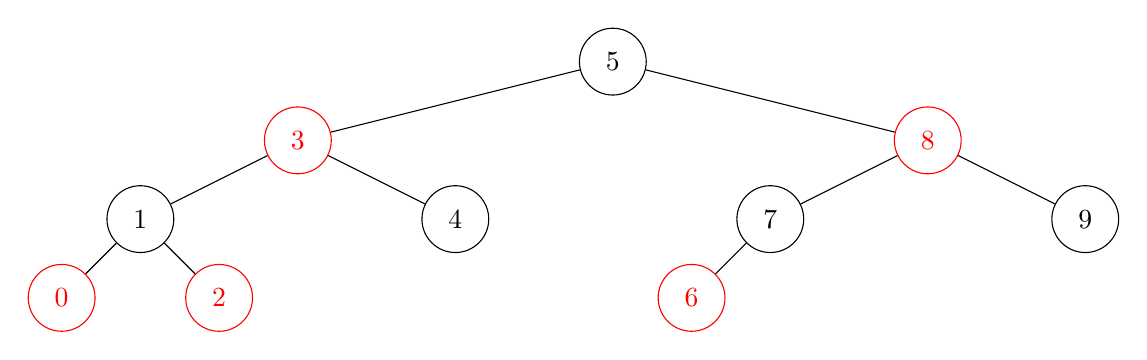
\begin{tikzpicture}[>=stealth]
    \node[ell] (a) at (8,3) {5};
    \node[red,ell] (b) at (4,2) {3};
    \node[red,ell] (c) at (12,2) {8};
    \node[ell] (d) at (2,1) {1};
    \node[ell] (e) at (6,1) {4};
    \node[ell] (f) at (10,1) {7};
    \node[ell] (g) at (14,1) {9};
    \node[red,ell] (h) at (1,0) {0};
    \node[red,ell] (i) at (3,0) {2};
    \node[red,ell] (j) at (9,0) {6};

    \draw [] (a) to []node[]{} (b);
    \draw [] (a) to []node[]{} (c);
    \draw [] (b) to []node[]{} (d);
    \draw [] (b) to []node[]{} (e);
    \draw [] (c) to []node[]{} (f);
    \draw [] (c) to []node[]{} (g);
    \draw [] (d) to []node[]{} (h);
    \draw [] (d) to []node[]{} (i);
    \draw [] (f) to []node[]{} (j);
\end{tikzpicture}
\end{problem}
\pagebreak
\begin{problem}{5}
    Remove the node with key `12' from the following red-black tree\\\\
    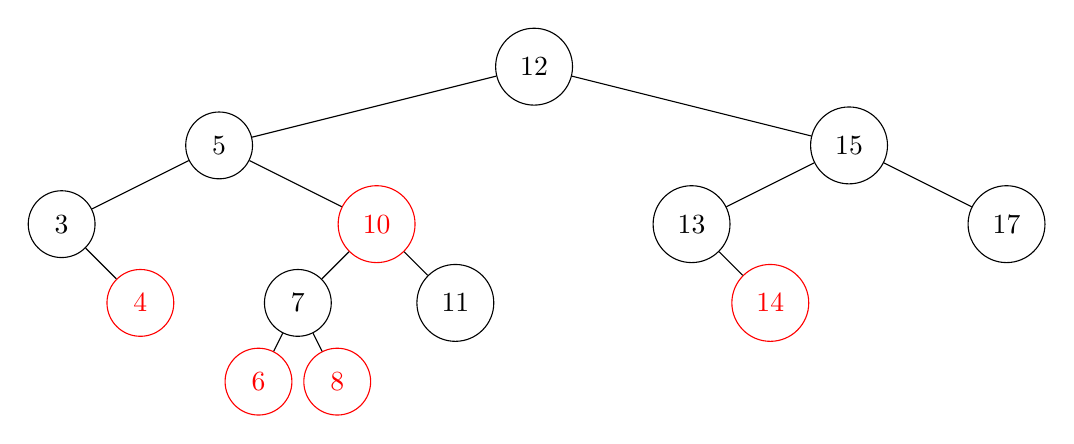
\begin{tikzpicture}[>=stealth]
        \node[ell] (a) at (8,3) {12};
        \node[ell] (b) at (4,2) {5};
        \node[ell] (c) at (12,2) {15};
        \node[ell] (d) at (2,1) {3};
        \node[red,ell] (e) at (6,1) {10};
        \node[ell] (f) at (10,1) {13};
        \node[ell] (g) at (14,1) {17};
        \node[red,ell] (h) at (3,0) {4};
        \node[ell] (i) at (5,0) {7};
        \node[ell] (j) at (7,0) {11};
        \node[red,ell] (k) at (11,0) {14};
        \node[red,ell] (l) at (4.5,-1) {6};
        \node[red,ell] (m) at (5.5,-1) {8};
    
        \draw [] (a) to []node[]{} (b);
        \draw [] (a) to []node[]{} (c);
        \draw [] (b) to []node[]{} (d);
        \draw [] (b) to []node[]{} (e);
        \draw [] (c) to []node[]{} (f);
        \draw [] (c) to []node[]{} (g);
        \draw [] (d) to []node[]{} (h);
        \draw [] (e) to []node[]{} (i);
        \draw [] (e) to []node[]{} (j);
        \draw [] (f) to []node[]{} (k);
        \draw [] (i) to []node[]{} (l);
        \draw [] (i) to []node[]{} (m);
    \end{tikzpicture}
    \\\\Case 6, replace z by its successor y, y takes color of z\\\\
    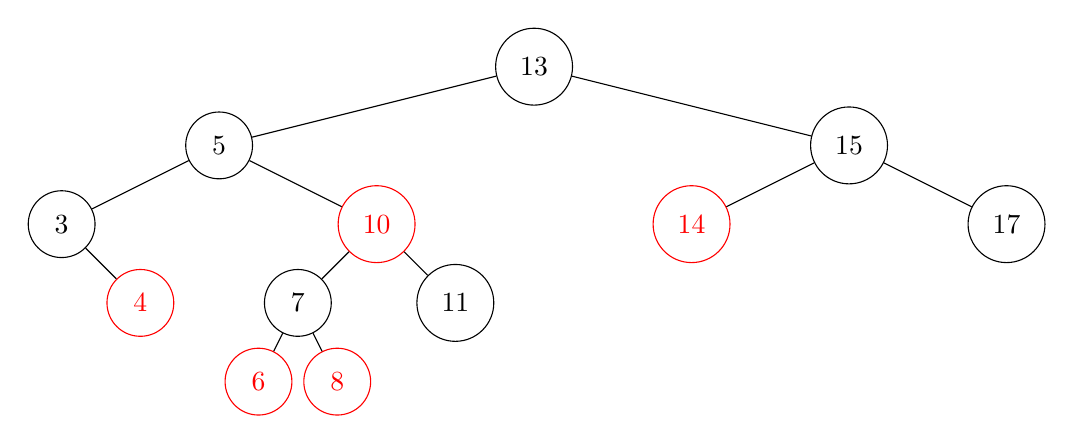
\begin{tikzpicture}[>=stealth]
        \node[ell] (a) at (8,3) {13};
        \node[ell] (b) at (4,2) {5};
        \node[ell] (c) at (12,2) {15};
        \node[ell] (d) at (2,1) {3};
        \node[red,ell] (e) at (6,1) {10};
        \node[red,ell] (f) at (10,1) {14};
        \node[ell] (g) at (14,1) {17};
        \node[red,ell] (h) at (3,0) {4};
        \node[ell] (i) at (5,0) {7};
        \node[ell] (j) at (7,0) {11};
        \node[red,ell] (l) at (4.5,-1) {6};
        \node[red,ell] (m) at (5.5,-1) {8};
    
        \draw [] (a) to []node[]{} (b);
        \draw [] (a) to []node[]{} (c);
        \draw [] (b) to []node[]{} (d);
        \draw [] (b) to []node[]{} (e);
        \draw [] (c) to []node[]{} (f);
        \draw [] (c) to []node[]{} (g);
        \draw [] (d) to []node[]{} (h);
        \draw [] (e) to []node[]{} (i);
        \draw [] (e) to []node[]{} (j);
        \draw [] (i) to []node[]{} (l);
        \draw [] (i) to []node[]{} (m);
    \end{tikzpicture}
    \\\\Case 3, recolor child\\\\
    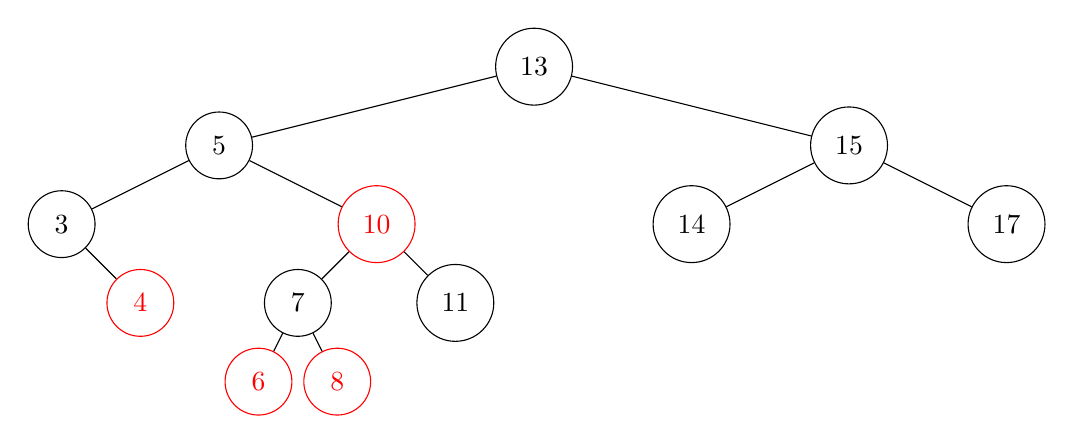
\begin{tikzpicture}[>=stealth]
        \node[ell] (a) at (8,3) {13};
        \node[ell] (b) at (4,2) {5};
        \node[ell] (c) at (12,2) {15};
        \node[ell] (d) at (2,1) {3};
        \node[red,ell] (e) at (6,1) {10};
        \node[ell] (f) at (10,1) {14};
        \node[ell] (g) at (14,1) {17};
        \node[red,ell] (h) at (3,0) {4};
        \node[ell] (i) at (5,0) {7};
        \node[ell] (j) at (7,0) {11};
        \node[red,ell] (l) at (4.5,-1) {6};
        \node[red,ell] (m) at (5.5,-1) {8};
    
        \draw [] (a) to []node[]{} (b);
        \draw [] (a) to []node[]{} (c);
        \draw [] (b) to []node[]{} (d);
        \draw [] (b) to []node[]{} (e);
        \draw [] (c) to []node[]{} (f);
        \draw [] (c) to []node[]{} (g);
        \draw [] (d) to []node[]{} (h);
        \draw [] (e) to []node[]{} (i);
        \draw [] (e) to []node[]{} (j);
        \draw [] (i) to []node[]{} (l);
        \draw [] (i) to []node[]{} (m);
    \end{tikzpicture}

\end{problem}

% --------------------------------------------------------------
%     You don't have to mess with anything below this line.
% --------------------------------------------------------------
 
\end{document}